\documentclass{beamer}

% \usepackage[pantone312,english]{wwustyle-nometa}
\usepackage[pantone312]{wwustyle}

\usepackage[ngerman]{babel}
\usepackage[utf8]{inputenc}
\usepackage[T1]{fontenc}
\usepackage{pgfplotstable}
\usepackage{booktabs}
\usepackage{array}
\usepackage{pgfplots}
\usepackage{lmodern}
\usepackage{media9}

% Uncomment the following two lines if you want to prepare your document for
% the fast mode.
% \usetikzlibrary{external}
% \tikzexternalize

% If frametitle is empty and subsection is not empty, use subsection as frame title
% If frametitle is empty and subsection is empty, use section as frame title
\makeatletter
  \CheckCommand*\beamer@checkframetitle{%
    \@ifnextchar\bgroup\beamer@inlineframetitle{}}
  \renewcommand*\beamer@checkframetitle{%
    \global\let\beamer@frametitle\relax\@ifnextchar%
    \bgroup\beamer@inlineframetitle{}}
\makeatother

\addtobeamertemplate{frametitle}{
  \ifx\insertframetitle\empty
    \ifx\insertframesubtitle\empty
      \ifx\insertsubsection\empty
        \frametitle{\insertsectionhead}
      \else
        \frametitle{\insertsubsectionhead}
      \fi
    \else
    \fi
    \else
    \fi
 }{}

\pgfplotstableset{% global config, for example in the preamble
  every head row/.style={before row=\toprule,after row=\midrule},
  every last row/.style={after row=\bottomrule}
}

% for each new section, show toc with highlighted section name
\AtBeginSection[]
{
  \begin{frame}
    \frametitle{Inhalt}
    \tableofcontents[currentsection]
  \end{frame}
}

\author{Robin, Johannes, Alexander}
\title{Emotionserkennung}
% \institutelogo{Logo on title frame}
% \institutelogosmall{Logo on other frames}
\subtitle{Klassifikation von Action-Units anhand von Landmarks}
\date{8. September 2016}

\begin{document}

%%%%%%%%%%%%%%% WWUstyle "fast" mode %%%%%%%%%%%%%%%%%%%%%
% Do the following steps in order to speed up the compilation time of your
% presentation:
%
% 1. Include the externalization tikz library in the preamble of your document.
%    This is always recommended if you are using tikz in your document.
% 2. Uncomment the \wwupreparefastmode command below
% 3. Compile your document with command line option '-shell-escape',
%    e.g.: 'pdflatex -shell-escape beamer.tex'
% 4. Comment (or delete) the \wwupreparefastmode
% 5. Add option 'fast' to the 'wwustyle' package declaration line.
% 6. Be happy!

% \wwupreparefastmode


\begin{frame}[plain]
  \maketitle
\end{frame}
\begin{frame}
  \frametitle{Inhalt}
  \tableofcontents
\end{frame}

\section{Aufgabenstellung}
\subsection{Eingabedaten}
\begin{frame}
  \begin{center}
  \includemedia[
      activate=onclick,
      height=0.8\textheight
  ]{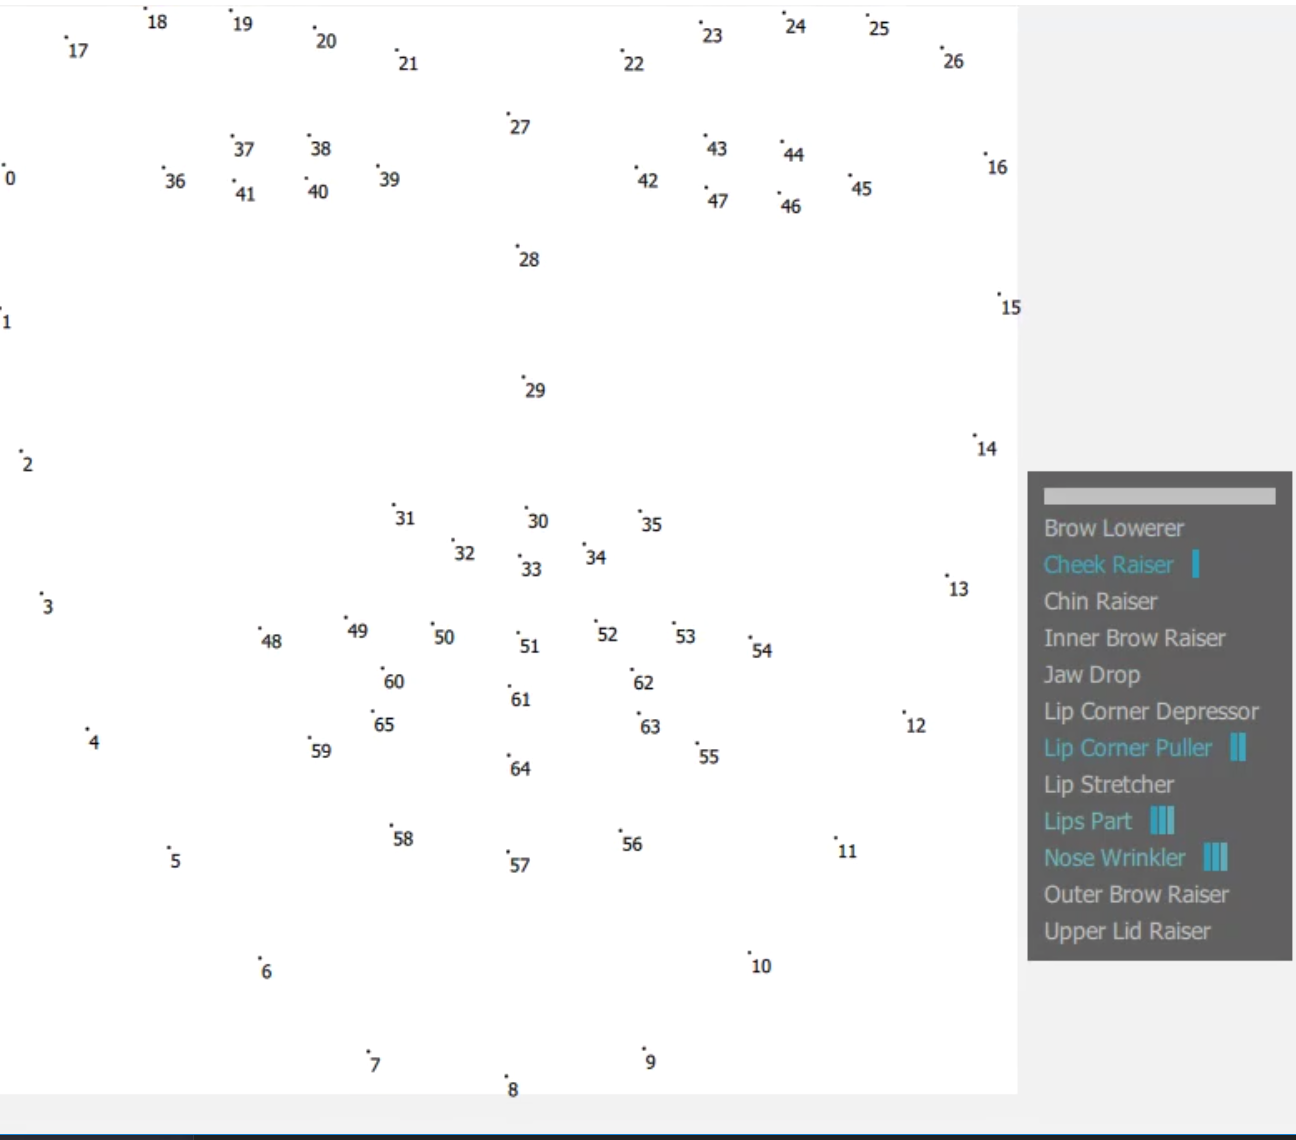
\includegraphics{aufgabenstellung.png}}{aufgabenstellung.swf}
  \end{center}
\end{frame}

\subsection{Ziel}
\begin{frame}
  \begin{block}{Ziel}
    Trainieren eines Klassifikators, der in der Lage ist aus eingehenden Landmarks die aktivierten Action Units zu erkennen.
  \end{block}
  \pause
\end{frame}

\section{Pipeline}
\subsection{Normalisierung}
\begin{frame}
  \begin{itemize}
    \item Verschiedene Personen unter den Eingabevideos
    \item Problem: Varianz durch unterschiedliche Größe und Rotation der Daten
    \item Lösung: Normalisierung der Daten
  \end{itemize}
\end{frame}

\subsection{Feature Extraction}
\begin{frame}
  \begin{itemize}
    \item Aufgabe: Extrahierung aussagekräftiger Merkmale aus den Landmarks
    \item Beispiel: Relation der Landmarks zueinander
  \end{itemize}
\end{frame}

\begin{frame}
  \begin{itemize}
    \item FeatureExtractor als Aggregate
  \end{itemize}
  \begin{center}
    \includegraphics[height=0.5\textheight]{feature_extractor.png}
  \end{center}
\end{frame}

\begin{frame}
  \begin{itemize}
    \item XYFeatureExtraction
    \item OrientationExtraction
    \item DistanceExtraction
    \item MaskedFeatureExtraction
    \item TimeFeatureExtraction
  \end{itemize}
\end{frame}

\subsection{PCA}
\begin{frame}
  \begin{itemize}
    \item bla
  \end{itemize}
\end{frame}

\subsection{Feature Scaling}
\begin{frame}
  \begin{itemize}
    \item bla
  \end{itemize}
\end{frame}

\subsection{Klassifikation}
\subsubsection{SVM}
\subsubsection{Andere Klassifikatoren}
\begin{frame}
  % \frametitle{Folientitel sollten kurz und prägnant sein}
  \begin{block}{Hervorhebungen}
    \textbf{Wenn man Dinge hervorheben möchte nutzt man entweder Fettdruck,}
    \textit{ kursive Schrift} \alert{ oder das Schlüsselwort ``alert''}.
  Auch ``itemize''-Umgebungen werden von der Stilvorlage überschrieben:
  \end{block}
  \pause
  \begin{itemize}
    \item So wird sichergestellt,
    \item dass alle Elemente der Präsentation
    \item dieselbe Farbe nutzen.
  \end{itemize}
\end{frame}

\subsection{Zusammenfassung}
\begin{frame}
  \begin{center}
    \includegraphics[height=0.8\textheight]{pipeline.png}
  \end{center}
\end{frame}

\section{Evaluation}
\subsection{Methodik}
\begin{frame}
  % \frametitle{Ein Alerted-Block}
  \begin{alertblock}{Achtung!}
    Hier kommt Rot ins Spiel!
  \end{alertblock}
  \begin{exampleblock}{Beispiel}
    Hier kommt Grün ins Spiel!
  \end{exampleblock}
\end{frame}

\subsection{Ergebnisse}
\begin{frame}
  \begin{table}
  \centering
  \pgfplotstabletypeset[
  col sep=comma,
  columns/Klassifikator/.style={string type}
  ]{data/tab_prec_recall.csv}
  \caption{Vergleich der Klassifikatoren}
  \label{tab:prec-recall}
  \end{table}
\end{frame}

\begin{frame}[plain]
\begin{figure}
\begin{tikzpicture}
  \begin{axis}[
    width=\textwidth,
    height=\textheight,
    xmin=0, xmax=1,
    ymin=0, ymax=1,
    xlabel={$1-\text{Precision}$},
    ylabel={Recall},
    domain=0:1,
    % legend entries={Sachen},
    % legend pos=north west
  ]
  \addplot table[only marks, col sep=comma] {data/plt_prec_recall.csv};
  \end{axis}
\end{tikzpicture}
\caption{Precision-Recall-Kurve}
\label{fig:prec-recall}
\end{figure}
\end{frame}

\end{document}
